\documentclass{standalone}
\usepackage{tikz}
\begin{document}
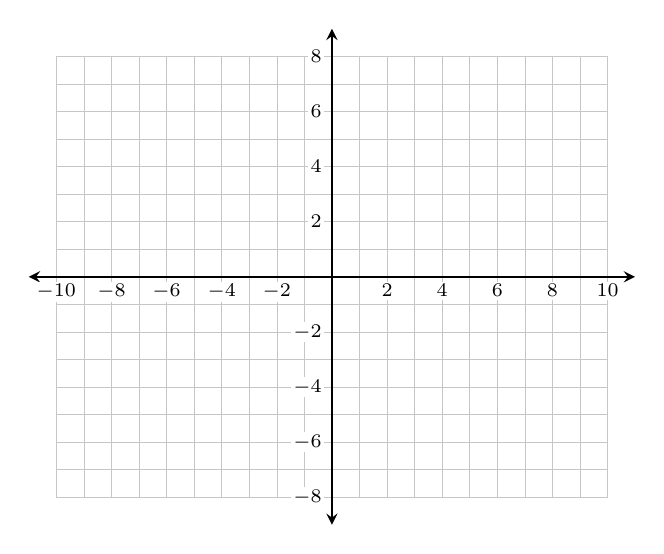
\begin{tikzpicture}[>=stealth, scale=0.35]
  % Blank coordinate plane: unit grid from -10 to 10 horizontally and
  % -8 to 8 vertically
  \draw[gray!45, very thin] (-10,-8) grid (10,8);
  % Axes, drawn past the grid so both arrow tips clear it
  \draw[<->, thick] (-11,0) -- (11,0);
  \draw[<->, thick] (0,-9) -- (0,9);
  % Tick labels at every even value, with a white halo so the grid
  % lines behind them stay out of the way
  \foreach \x in {-10,-8,-6,-4,-2,2,4,6,8,10} {
    \node[below, font=\scriptsize, fill=white, inner sep=1pt] at (\x,-0.15) {$\x$};
  }
  \foreach \y in {-8,-6,-4,-2,2,4,6,8} {
    \node[left, font=\scriptsize, fill=white, inner sep=1pt] at (-0.25,\y) {$\y$};
  }
\end{tikzpicture}
\end{document}
